\documentclass{beamer}
\usetheme{focus}
% Add option [numbering=none] to disable the footer progress bar
% Add option [numbering=fullbar] to show the footer progress bar as always full with a slide count
% Uncomment to enable the ice-blue theme
%\definecolor{main}{RGB}{92, 138, 168}
%\definecolor{background}{RGB}{240, 247, 255}
\usepackage{booktabs} % Required for better table rules
\usepackage{enumerate}
\usepackage{xcolor, listings}

\title{
\includegraphics[scale=.45]{img/dpdk_logo.png}}
%\subtitle{ein kurzer Überblick}
\titlegraphic{
\includegraphics[scale=.1]{img/tu_ilmenau_logo.png}}
%\institute{Institute Name \\ Institute Address}
\date{6.5.2021}

\begin{document}
\begin{frame}
    \maketitle % Automatically created using the information in the commands above
\end{frame}

\begin{frame}{Überblick über DPDK}
    \begin{itemize}
        \item Sammlung von Bibliotheken
        \item 2010 von Intel veröffentlicht
        \item freie OpenSource Lizenz
        \item unterstützt alle wichtigen CPU-Architekturen und NICs
    \end{itemize}
    \note{
        NIC = Network Interface Card  á Netzwerkkarte
    }
\end{frame}

\begin{frame}{Grundlegendes Problem}
    \begin{itemize}
        \item viele Engpässe verhindern Verarbeitung von Paketen
        \item Bottleneck im Linux Kernel selbst
        \item[$\rightarrow$] Kernel-Bypass
        \item[$\rightarrow$] Anwendungen kommunizieren direkt mit Netzwerkgeräten
    \end{itemize}
\end{frame}

\begin{frame}{Fahrplan für Heute}
    \tableofcontents
\end{frame}

%----------------------------------------------------------------------------------------
%	 SECTION
%----------------------------------------------------------------------------------------
\section{DPDK vs. Kernel Processing}
\begin{frame}{Linux Kernel ohne DPDK}
    \begin{columns}
        \column{0.4\textwidth}
        \begin{figure}[h]
            \centering
            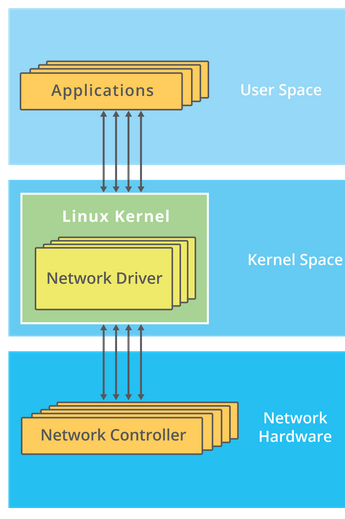
\includegraphics[width=\linewidth]{img/kernel_without_dpdk.png}
        \end{figure}
        \column{0.5\textwidth}
        \begin{itemize}
            \item Netzwerkkarte sendet Paket zu Warteschlange
            \item per DMA in Hauptspeicher kopieren
            \item Kernel weißt Puffer zu \alert{Interrupts!}
            \item Paket aus Puffer in User Space übertragen
        \end{itemize}
    \end{columns}
    \note{
        - Empfängt eine Netzwerkkarte ein Paket sendet sie es an eine Empfangswarteschlange
        - Von dort wird das Paket über DMA-Mechanismus (Direct Memory Access) in den Hauptspeicher kopiert.
        - Danach wird das System über das neue Paket benachrichtigt und das Paket von Linux einem Puffer (sk\_buff) zugewiesen. Für jedes neue Paket wird im System ein oder mehrere Interrupts erzeugt.
        - Das Paket muss dann noch in den User Space übetragen (kopiert) werden
    }
\end{frame}

\begin{frame}{Linux Kernel mit DPDK}
    \begin{columns}
        \column{0.4\textwidth}
        \begin{figure}[h]
            \centering
            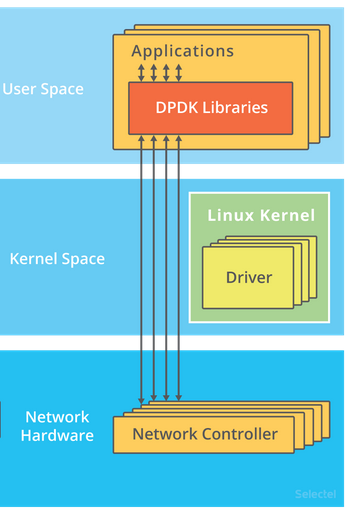
\includegraphics[width=\linewidth]{img/kernel_and_dpdk.png}
        \end{figure}
        \column{0.5\textwidth}
        \begin{itemize}
            \item Netzwerkports vom Kernel getrennt/ungebunden
            \item Eingehende Pakete gehen in Ringpuffer
            \item Wenn Puffer neue Paketdeskriptoren enthält, verweis auf die DPDK-Paketpuffer
            \item Wenn Ringpuffer keine Pakete enthält, stelle Netzwerkgeräte in Warteschlange
            \item erfordert Konfiguration von \alert{hugepages}
        \end{itemize}
    \end{columns}
    \note{
        - DPDK durch Treiber direkt mit Port gebunden
        - Um die Bindung eines Geräts an einen Treiber aufzuheben, muss die Busnummer des Geräts in die unbind-Datei geschrieben werden. Um ein Gerät an einen anderen Treiber zu binden, muss die Busnummer in dessen Bind-Datei geschrieben werden.
        - Ports von den Treibern vfio_pci, igb_uio oder uio_pci_generic verwaltet
        - Treiber ermöglichen es, mit Geräten im User-Space zu interagieren
        - Kommunikation über DPDK-Poll-Mode-Treiber (PMD); für alle unterstützten Netzwerkkarten und virtuellen Geräte möglich
        1. Eingehende Pakete gehen in einen Ringpuffer. Die Anwendung prüft diesen Puffer periodisch auf neue Pakete.
        2. Wenn der Puffer neue Paketdeskriptoren enthält, verweist die Anwendung mit Hilfe der Zeiger in den Paketdeskriptoren auf die DPDK-Paketpuffer im speziell zugewiesenen Speicherpool.
        3. Wenn der Ringpuffer keine Pakete enthält, wird die Anwendung die Netzwerkgeräte unter dem DPDK in eine Warteschlange stellen und dann erneut auf den Ring verweisen.
    }
\end{frame}

%----------------------------------------------------------------------------------------
%	 SECTION
%----------------------------------------------------------------------------------------
\section{DPDK Aufbau}
\begin{frame}{DPDK-Core}
    \centering\huge
    \begin{tabular}{|c|}
        \hline
        EAL     \\\hline
        MBUF    \\\hline
        MEMPOOL \\\hline
        RING    \\\hline
        TIMER   \\\hline
    \end{tabular}
\end{frame}

\begin{frame}{Environment Abstraction Layer (EAL)}
    \begin{itemize}
        \item Satz von Programmierwerkzeugen
        \item bindet Anwendungen an DPDK
        \item alle Anwendungen müssen Header Dateien der EAL enthalten
    \end{itemize}
\end{frame}

\begin{frame}{Environment Abstraction Layer (EAL)}
    die häufigsten/wichtigsten Header\footnote{\href{http://dpdk.org/doc/guides/prog_guide/env_abstraction_layer.html}{http://dpdk.org/doc/guides/prog\_guide/env\_abstraction\_layer.html}}:
    \begin{description}
        \item[rte\_lcore.h] verwaltet Prozessorkerne und Sockel
        \item[rte\_memory.h] verwaltet Speicher
        \item[rte\_pci.h] Schnittstelle für den Zugriff auf PCI-Adressraum
        \item[rte\_debug.h] Trace- und Debug-Funktionen
        \item[rte\_interrupts.h] verarbeitet Interrupts
    \end{description}
\end{frame}

%----------------------------------------------------------------------------------------
%	 SECTION
%----------------------------------------------------------------------------------------
\section{Paketrepräsentation}
\begin{frame}{Kurz und knapp}
    \begin{itemize}
        \item Nutzung von PMDs (Poll Mode Drivers)\footnote{\href{http://doc.dpdk.org/guides/prog_guide/poll_mode_drv.html}{http://doc.dpdk.org/guides/prog\_guide/poll\_mode\_drv.html}}
        \item Pakete werden in Speicherblöcken untergebracht
        \item diese Blöcke nennt man "Buffer" (konkret: Mbuf)\footnote{\href{http://doc.dpdk.org/guides/prog_guide/mbuf_lib.html}{http://doc.dpdk.org/guides/prog\_guide/mbuf\_lib.html}}
              \begin{itemize}
                  \item nicht zu verwechseln mit Ring Buffer!
              \end{itemize}
    \end{itemize}
    \note{
        * Wie kann man auf Paket vom Code zugreifen --> PMD (ganz grob)
        * Wie wird Paket in Code repräsentiert? --> Buffer, ist ein Speicher
        * Nun Mbuf, Mempool näher erklären
    }
\end{frame}

\begin{frame}{Mempool}
    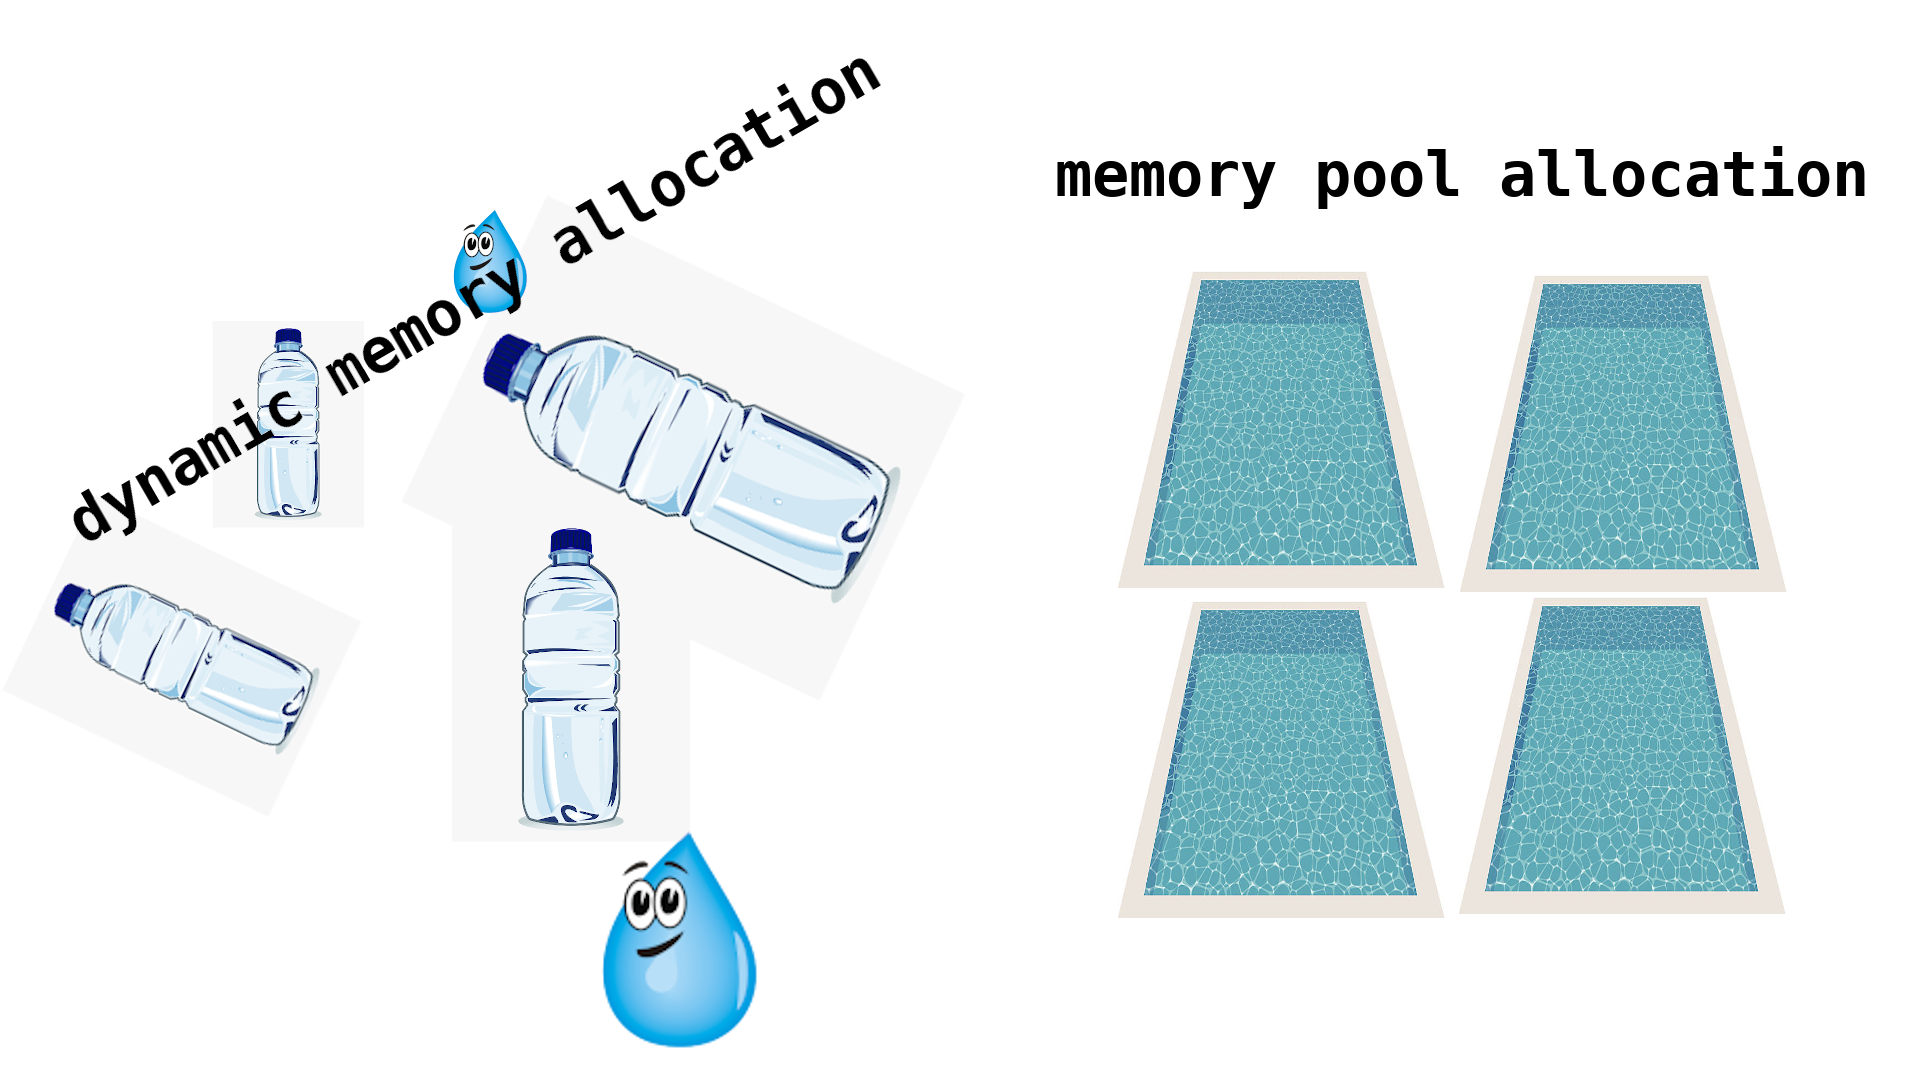
\includegraphics[width=\linewidth]{img/mempool.png}
    \vspace*{\fill}
    \href{https://en.wikipedia.org/wiki/Memory_pool}{https://en.wikipedia.org/wiki/Memory\_pool}\\
    \href{http://doc.dpdk.org/guides/prog_guide/mempool_lib.html}{http://doc.dpdk.org/guides/prog\_guide/mempool\_lib.html}
    \note{
        * Bevor: brauchen Speicherplatz
        * Möglichk. Allok.:
        --> dynamisch (new, malloc)
        --> fixed-sized, mempool genannt
        * Memory pool alloc ist besser... (fragmentierung)
        * dazu Mempool Library in dpdk.
        * beinhaltet sog. Mempool allocator, also ein Ding was diese Mempool allokation durchführt
        * Speicher müssen wir selbst holen, mithlife dieser Bibliothek
        * für zB. Mbuf nutzen
    }
\end{frame}

\begin{frame}{Mempool: Ring}
    \begin{itemize}
        \item Mempool \textbf{nutzt} intern \textbf{rte\_ring} (Queue)
              \begin{itemize}
                  \item speichert dort Referenzen auf Speicherbereiche
              \end{itemize}
    \end{itemize}
\end{frame}

\begin{frame}{Mempool: Local Cache}
    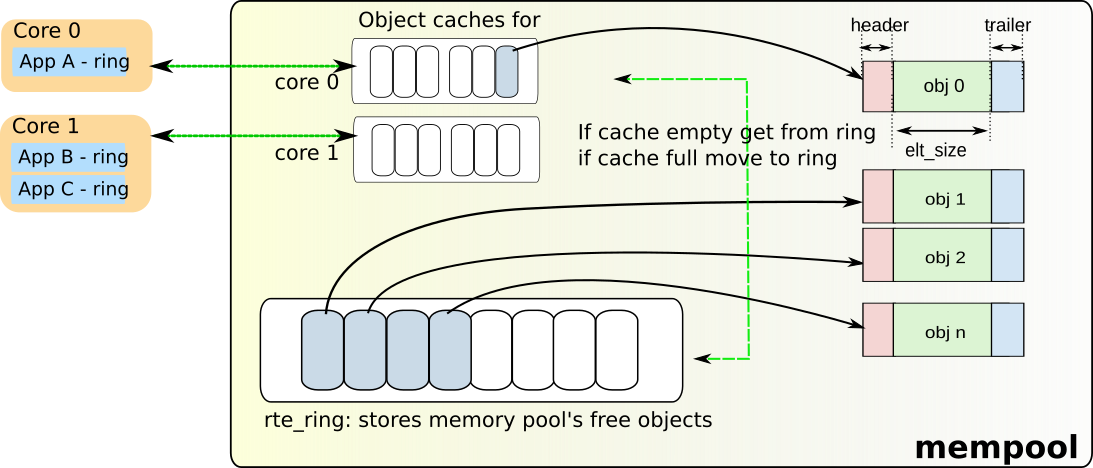
\includegraphics[width=\linewidth]{img/mempool2.png}
    \note{
        * local cache für jeden CPU-Kern
        * bulk requests
        * weniger locks des hauptrings
        * selbst konfigurieren: THIS INTERNAL CACHE CAN BE ENABLED ... AT CREATION OF POOL
    }
\end{frame}

\begin{frame}{Mbuf}
    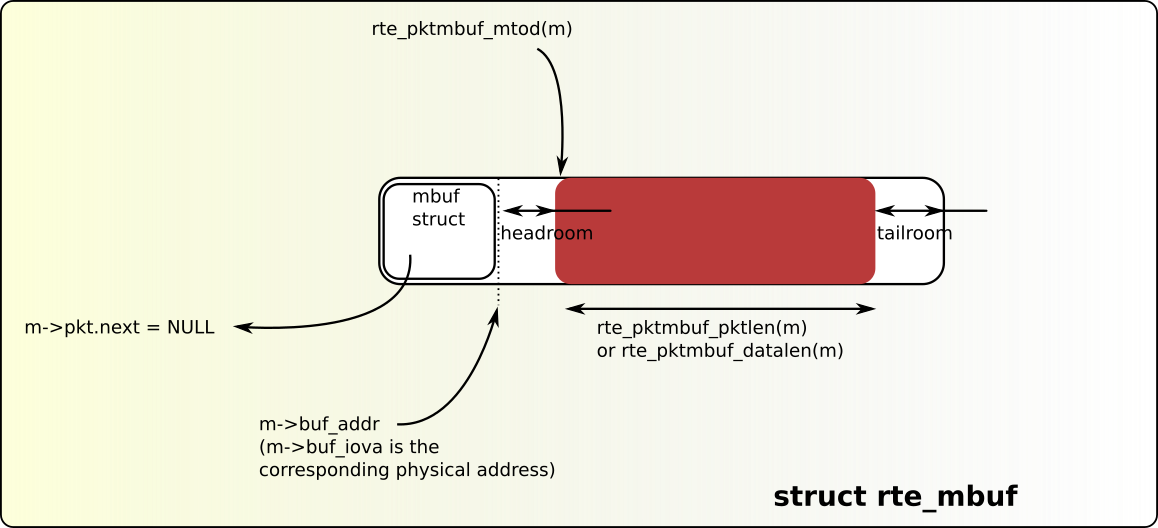
\includegraphics[width=\linewidth]{img/mbuf1.png}
    \note{
        * Adressraum (Buffer), der Metadaten und Paketdaten selbst enthält.
        * Metadaten und Paketdaten in einem Buffer
        * Für Buffer wird Datenstruktur mbuf verwendet.
    }
\end{frame}

\begin{frame}{Mbuf: Indirect buffer}
    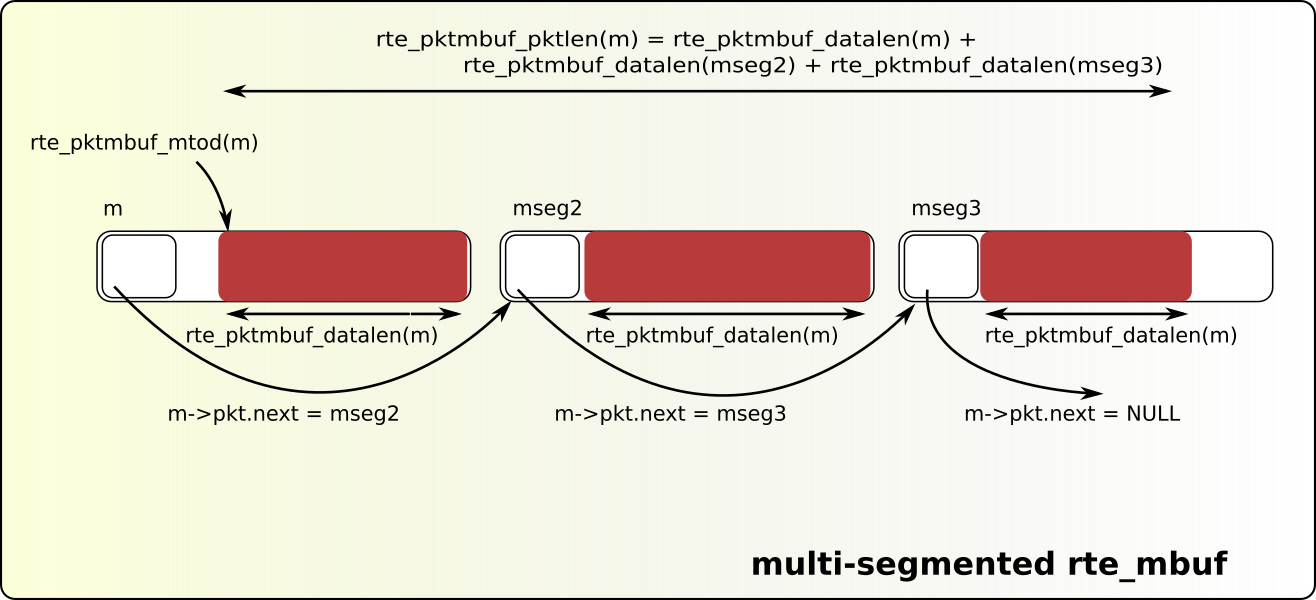
\includegraphics[width=\linewidth]{img/mbuf2.png}
    \note{
        * Für goße Pakete kann man mehrere Buffer aneinanderhängen
        * normalerweise Buffer: Zwischenspeicher. Trifft hier ja auch zu, weil Pakete kurz gespeichert und dann weitergegeben werden
    }
\end{frame}

\begin{frame}{Verwalten von Warteschlangen}
    \begin{itemize}
        \item Queue durch Bibliothek \textbf{rte\_ring}\footnote{\href{https://doc.dpdk.org/guides-16.07/prog_guide/ring_lib.html}{https://doc.dpdk.org/guides-16.07/prog\_guide/ring\_lib.html}} implementiert
        \item aus FreeBSD Ringpuffer\footnote{\href{https://svnweb.freebsd.org/base/release/8.0.0/sys/sys/buf_ring.h}{https://svnweb.freebsd.org/base/release/8.0.0/sys/sys/buf\_ring.h}} entwickelt
        \item sperrfreier Ringpuffer nach FIFO-Prinzip
        \item Zeiger mit vier Kategorien
              \begin{itemize}
                  \item prod\_tail
                  \item prod\_head
                  \item cons\_tail
                  \item cons\_head
              \end{itemize}
    \end{itemize}
    \note{
        - Ringpuffer ist eine Tabelle mit Zeigern für Objekte, die im Speicher abgelegt werden können
        - Prods ist Abkürzung für Producer, cons für Consumer
        - Producer ist Prozess, der zu bestimmten Zeitpunkt Daten in den Puffer schreibt
        - Consumer ist Prozess, der Daten aus dem Puffer entfernt
        - Tail ist der Ort, an dem Schreiben auf den Ringpuffer stattfindet
        - Kopf ist der Ort, von dem der Puffer gelesen wird
    }
\end{frame}

\begin{frame}{Verwalten von Warteschlangen}
    \begin{columns}[T, onlytextwidth]
        \column{0.5\textwidth}
        Vorteile
        \begin{itemize}
            \item Daten extrem schnell in Puffer schreiben
            \item viel seltener Cache-Misses
        \end{itemize}
        \column{0.5\textwidth}
        Nachteil
        \begin{itemize}
            \item feste unveränderliche Größe
            \item höherer Speicherverbrauch
        \end{itemize}
    \end{columns}
    \note{
        Vorteile:
        - viel seltener Cache-Misses, da Zeiger in einer Tabelle gespeichert werden
        Nachteile:
        - feste unveränderliche Größe, die nicht im laufenden Betrieb erhöht werden kann
        - bei der Arbeit mit der Ringstruktur viel mehr Speicher verbraucht als bei einer verknüpften Warteschlange, da der Puffer immer die maximale Anzahl von Zeigern verwendet
    }
\end{frame}

\begin{frame}{Revision: Pakete verarbeiten}
    Programmierer sorgt dafür, dass:
    \begin{enumerate}
        \item alles richtig \textbf{konfiguriert} ist
        \item \textbf{PMD} die Pakete holt
        \item Speicher vom \textbf{Mempool} geholt wird
        \item Mithilfe des Mempool ein \textbf{Mbuf} erzeugt wird
        \item in den Pakete reingesteckt werden
    \end{enumerate}
    \vspace{.5cm} Details stehen in der Dokumentation! \\
    Es gibt viele verschiedene Wege, Beispielprogramme geben Orientierung.
    \note{
        * PMD holt Pakete
        * Programmierer:
        * holt Speicher vom Mempool
        * intern stehen Speicheradressen in einem Ring
        * erstellt mithilfe dessen einen Mbuf
        * steckt Pakete in Mbuf hinein
        * Mit Paketen arbeiten
    }
\end{frame}

\begin{frame}{Zusammenhang der Komponenten}
    \centering
    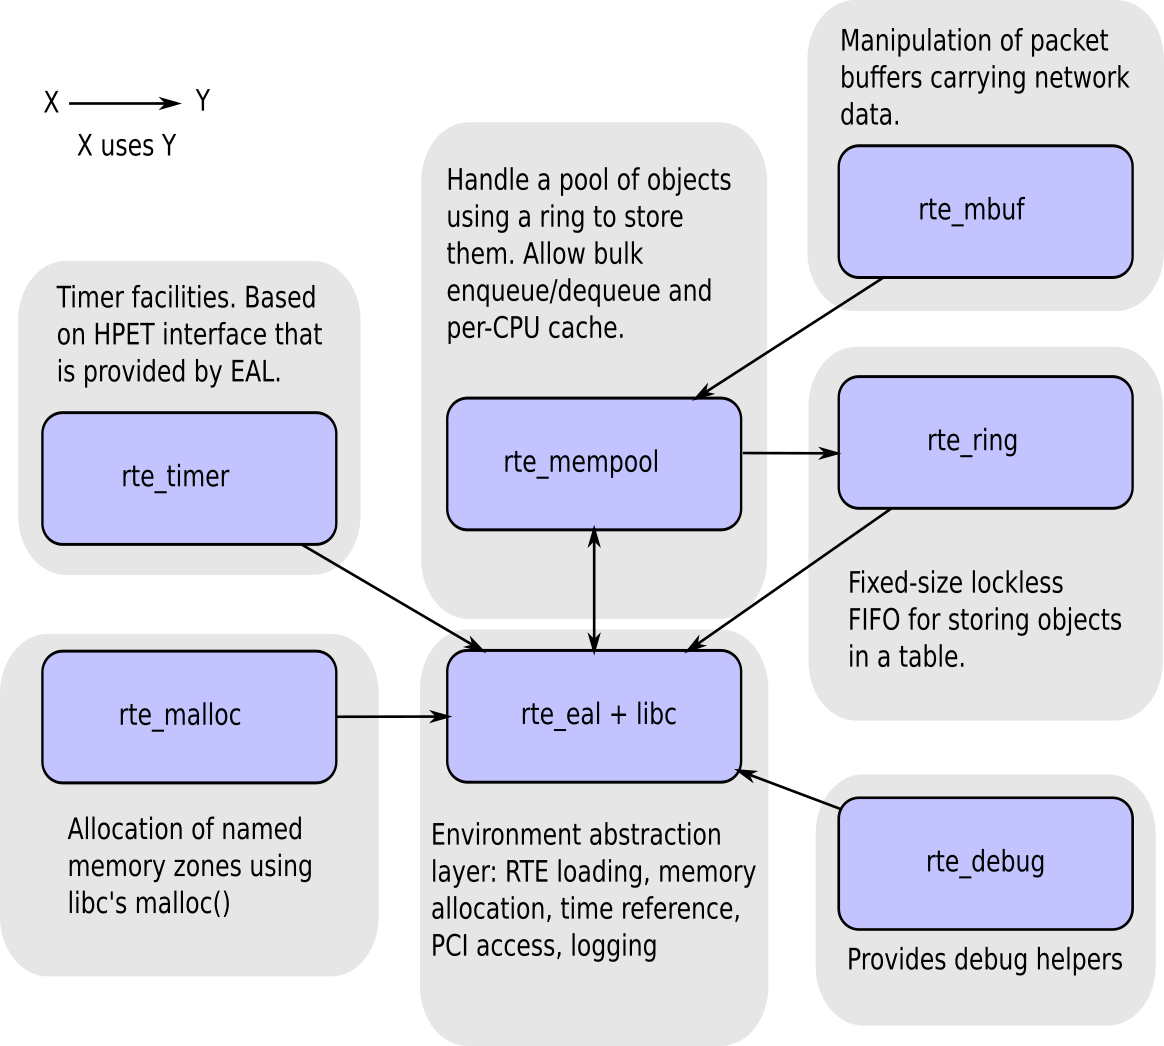
\includegraphics[width=.9\textheight]{img/architecture.png}
\end{frame}

\begin{frame}{Was sind Hugepages?}
    \begin{itemize}
        \item Memory management unit (\textbf{MMU}):
              \begin{itemize}
                  \item Teil der CPU,
                  \item realisiert Zuordnung VA \(\mapsto\) PA
              \end{itemize}
        \item Translation lookaside buffer (\textbf{TLB}):
              \begin{itemize}
                  \item Speichert oft genutzte Einträge
                  \item schneller Zugriff auf Einträge
                  \item bei vielen Einträgen ineffizient
              \end{itemize}
        \item größere Pages $\rightarrow$ weniger Einträge
        \item[\(\rightarrow\)] Inhalt ändert sich weniger oft
        \item[\(\Rightarrow\)] Zeiteffizienz erhöht!
    \end{itemize}
    \note{
        - Memory management unit (MMU): Teil der CPU, realisiert Zuordnung VA -> PA (Vorstellen als große Tabelle)
        - Translation lookaside buffer (TLB): Speichert oft genutzte Einträge dieser Tabelle (Cache)
        - -> an diese Einträge kommt man schneller ran
        - wenn viele Einträge benötigt werden, ändert sich Inhalt des TLBs ständig -> ineffizient
        - Verringerung der Einträge durch vergrößern der Pages (Pages werden huge) -> Inhalt des TLBs ändert sich nicht mehr so oft
        - Zeiteffizienz erhöht!
    }
\end{frame}

%----------------------------------------------------------------------------------------
%	 SECTION
%----------------------------------------------------------------------------------------
\section{Empfang und Senden von Paketen}
\begin{frame}{Vorbereitung}
    \begin{enumerate}
        \item runtime enviroment initialisieren
        \item mempool anwenden
        \item initialisiere NIC ports um tx/rx-Warteschlangen\footnote{\href{https://doc.dpdk.org/dts/test_plans/dynamic_queue_test_plan.html}{DPDK - Dynamic Queue Test}} zu erhalten und diesen Speicher zuweisen
        \item Definieren von mbuf und Anfordern von Speicher aus dem mempool
    \end{enumerate}
    \note{
        - wie zuvor beschrieben
        - konfigurieren: CPU Core, Netzwerkgeräte
        - falls Netzwerkgerät stoppt, stoppen alle Warteschlangen
    }
\end{frame}

\begin{frame}{Empfang Ablauf}
    \begin{enumerate}
        \item holt Paket vom NIC-Port zu mbuf
        \item analysiere mbuf und hole Paket
        \item Paket in Anwendung verwenden z.B. Inhalt des Paket drucken
    \end{enumerate}
\end{frame}

\begin{frame}{Senden Ablauf}
    \begin{enumerate}
        \item Paket in mbuf schreiben
        \item bewege mbuf zu tx Warteschlange
        \item Paket senden durch dpdk-api
    \end{enumerate}
\end{frame}

\begin{frame}{die wichtigsten Quellen}
    \begin{itemize}
        \item \href{http://doc.dpdk.org/guides/linux_gsg/}{DPDK Linux Guide} (Installation, Getting started)
        \item \href{http://doc.dpdk.org/guides/prog_guide/}{DPDK Programmer Guide} (für ausführliche Erklärungen)
              \begin{itemize}
                  \item \href{http://doc.dpdk.org/guides/prog_guide/ring_lib.html}{Ring Library}
                  \item \href{http://doc.dpdk.org/guides/prog_guide/mempool_lib.html}{Mempool Library}
                  \item \href{http://doc.dpdk.org/guides/prog_guide/mbuf_lib.html}{Mbuf Library}
                  \item \href{http://doc.dpdk.org/guides/prog_guide/poll_mode_drv.html}{Poll Mode Driver Library}
                  \item ...
              \end{itemize}
        \item \href{http://doc.dpdk.org/api/}{DPDK API Documentation} (zum Programmieren)
    \end{itemize}
\end{frame}

%----------------------------------------------------------------------------------------
%	 CLOSING/SUPPLEMENTARY SLIDES
%----------------------------------------------------------------------------------------
\begin{frame}[focus]
    Vielen Dank fürs Zuhören
\end{frame}
\appendix
\begin{frame}{Quellen}
    \href{https://www.dpdk.org/}{DPDK.org}

    \href{https://github.com/DPDK/dpdk}{github.com/DPDK/dpdk}

    \href{https://blog.selectel.com/introduction-dpdk-architecture-principles/}{blog.selectel.com}

    \href{https://www.net.in.tum.de/fileadmin/TUM/NET/NET-2014-08-1/NET-2014-08-1_15.pdf}{net.in.tum.de}

    \href{https://www.privateinternetaccess.com/blog/2016/01/linux-networking-stack-from-the-ground-up-part-1}{privateinternetaccess.com}

    \href{http://www.slideshare.net/garyachy/dpdk-44585840}{slideshare.net}

    \href{http://www.it-sobytie.ru/system/attachments/files/000/001/102/original/LinuxPiter-DPDK-2015.pdf}{it-sobytie.ru}

    \href{https://github.com/AltraMayor/gatekeeper/wiki}{github.com/AltraMayor/gatekeeper}

    \href{https://svnweb.freebsd.org}{svnweb.freebsd.org}

    \href{https://pcapplusplus.github.io/}{pcapplusplus.github.io}

    \href{https://en.wikipedia.org/wiki/Memory_pool}{wikipedia.org/wiki/Memory\_pool}

    \nocite{*} % Display all references regardless of if they were cited
    \bibliography{example.bib}
    \bibliographystyle{plain}
\end{frame}

\begin{frame}[focus]
    Zeit für eure Fragen
\end{frame}

\end{document}
